% Options for packages loaded elsewhere
\PassOptionsToPackage{unicode}{hyperref}
\PassOptionsToPackage{hyphens}{url}
%
\documentclass[
]{article}
\usepackage{amsmath,amssymb}
\usepackage{lmodern}
\usepackage{iftex}
\ifPDFTeX
  \usepackage[T1]{fontenc}
  \usepackage[utf8]{inputenc}
  \usepackage{textcomp} % provide euro and other symbols
\else % if luatex or xetex
  \usepackage{unicode-math}
  \defaultfontfeatures{Scale=MatchLowercase}
  \defaultfontfeatures[\rmfamily]{Ligatures=TeX,Scale=1}
\fi
% Use upquote if available, for straight quotes in verbatim environments
\IfFileExists{upquote.sty}{\usepackage{upquote}}{}
\IfFileExists{microtype.sty}{% use microtype if available
  \usepackage[]{microtype}
  \UseMicrotypeSet[protrusion]{basicmath} % disable protrusion for tt fonts
}{}
\makeatletter
\@ifundefined{KOMAClassName}{% if non-KOMA class
  \IfFileExists{parskip.sty}{%
    \usepackage{parskip}
  }{% else
    \setlength{\parindent}{0pt}
    \setlength{\parskip}{6pt plus 2pt minus 1pt}}
}{% if KOMA class
  \KOMAoptions{parskip=half}}
\makeatother
\usepackage{xcolor}
\usepackage[margin=1in]{geometry}
\usepackage{color}
\usepackage{fancyvrb}
\newcommand{\VerbBar}{|}
\newcommand{\VERB}{\Verb[commandchars=\\\{\}]}
\DefineVerbatimEnvironment{Highlighting}{Verbatim}{commandchars=\\\{\}}
% Add ',fontsize=\small' for more characters per line
\usepackage{framed}
\definecolor{shadecolor}{RGB}{248,248,248}
\newenvironment{Shaded}{\begin{snugshade}}{\end{snugshade}}
\newcommand{\AlertTok}[1]{\textcolor[rgb]{0.94,0.16,0.16}{#1}}
\newcommand{\AnnotationTok}[1]{\textcolor[rgb]{0.56,0.35,0.01}{\textbf{\textit{#1}}}}
\newcommand{\AttributeTok}[1]{\textcolor[rgb]{0.77,0.63,0.00}{#1}}
\newcommand{\BaseNTok}[1]{\textcolor[rgb]{0.00,0.00,0.81}{#1}}
\newcommand{\BuiltInTok}[1]{#1}
\newcommand{\CharTok}[1]{\textcolor[rgb]{0.31,0.60,0.02}{#1}}
\newcommand{\CommentTok}[1]{\textcolor[rgb]{0.56,0.35,0.01}{\textit{#1}}}
\newcommand{\CommentVarTok}[1]{\textcolor[rgb]{0.56,0.35,0.01}{\textbf{\textit{#1}}}}
\newcommand{\ConstantTok}[1]{\textcolor[rgb]{0.00,0.00,0.00}{#1}}
\newcommand{\ControlFlowTok}[1]{\textcolor[rgb]{0.13,0.29,0.53}{\textbf{#1}}}
\newcommand{\DataTypeTok}[1]{\textcolor[rgb]{0.13,0.29,0.53}{#1}}
\newcommand{\DecValTok}[1]{\textcolor[rgb]{0.00,0.00,0.81}{#1}}
\newcommand{\DocumentationTok}[1]{\textcolor[rgb]{0.56,0.35,0.01}{\textbf{\textit{#1}}}}
\newcommand{\ErrorTok}[1]{\textcolor[rgb]{0.64,0.00,0.00}{\textbf{#1}}}
\newcommand{\ExtensionTok}[1]{#1}
\newcommand{\FloatTok}[1]{\textcolor[rgb]{0.00,0.00,0.81}{#1}}
\newcommand{\FunctionTok}[1]{\textcolor[rgb]{0.00,0.00,0.00}{#1}}
\newcommand{\ImportTok}[1]{#1}
\newcommand{\InformationTok}[1]{\textcolor[rgb]{0.56,0.35,0.01}{\textbf{\textit{#1}}}}
\newcommand{\KeywordTok}[1]{\textcolor[rgb]{0.13,0.29,0.53}{\textbf{#1}}}
\newcommand{\NormalTok}[1]{#1}
\newcommand{\OperatorTok}[1]{\textcolor[rgb]{0.81,0.36,0.00}{\textbf{#1}}}
\newcommand{\OtherTok}[1]{\textcolor[rgb]{0.56,0.35,0.01}{#1}}
\newcommand{\PreprocessorTok}[1]{\textcolor[rgb]{0.56,0.35,0.01}{\textit{#1}}}
\newcommand{\RegionMarkerTok}[1]{#1}
\newcommand{\SpecialCharTok}[1]{\textcolor[rgb]{0.00,0.00,0.00}{#1}}
\newcommand{\SpecialStringTok}[1]{\textcolor[rgb]{0.31,0.60,0.02}{#1}}
\newcommand{\StringTok}[1]{\textcolor[rgb]{0.31,0.60,0.02}{#1}}
\newcommand{\VariableTok}[1]{\textcolor[rgb]{0.00,0.00,0.00}{#1}}
\newcommand{\VerbatimStringTok}[1]{\textcolor[rgb]{0.31,0.60,0.02}{#1}}
\newcommand{\WarningTok}[1]{\textcolor[rgb]{0.56,0.35,0.01}{\textbf{\textit{#1}}}}
\usepackage{graphicx}
\makeatletter
\def\maxwidth{\ifdim\Gin@nat@width>\linewidth\linewidth\else\Gin@nat@width\fi}
\def\maxheight{\ifdim\Gin@nat@height>\textheight\textheight\else\Gin@nat@height\fi}
\makeatother
% Scale images if necessary, so that they will not overflow the page
% margins by default, and it is still possible to overwrite the defaults
% using explicit options in \includegraphics[width, height, ...]{}
\setkeys{Gin}{width=\maxwidth,height=\maxheight,keepaspectratio}
% Set default figure placement to htbp
\makeatletter
\def\fps@figure{htbp}
\makeatother
\setlength{\emergencystretch}{3em} % prevent overfull lines
\providecommand{\tightlist}{%
  \setlength{\itemsep}{0pt}\setlength{\parskip}{0pt}}
\setcounter{secnumdepth}{-\maxdimen} % remove section numbering
\usepackage{booktabs}
\usepackage{longtable}
\usepackage{array}
\usepackage{multirow}
\usepackage{wrapfig}
\usepackage{float}
\usepackage{colortbl}
\usepackage{pdflscape}
\usepackage{tabu}
\usepackage{threeparttable}
\usepackage{threeparttablex}
\usepackage[normalem]{ulem}
\usepackage{makecell}
\usepackage{xcolor}
\ifLuaTeX
  \usepackage{selnolig}  % disable illegal ligatures
\fi
\IfFileExists{bookmark.sty}{\usepackage{bookmark}}{\usepackage{hyperref}}
\IfFileExists{xurl.sty}{\usepackage{xurl}}{} % add URL line breaks if available
\urlstyle{same} % disable monospaced font for URLs
\hypersetup{
  pdftitle={HW3-Trinath Sai Subhash Reddy-Pittala},
  pdfauthor={Subhash},
  hidelinks,
  pdfcreator={LaTeX via pandoc}}

\title{HW3-Trinath Sai Subhash Reddy-Pittala}
\author{Subhash}
\date{2023-03-22}

\begin{document}
\maketitle

\hypertarget{a.-create-two-small-datasets---flights.sm-and-flights.sm.aa-from-the-flights-data---both-variables-containing-only-the-following-variables-arr_delay-dep_delay-sched_dep_time-distance-air_time.-flights.sm-contains-data-from-all-carriers-and-flights.sm.aa-contains-only-data-from-aa-carrier.}{%
\subsubsection{A. Create two ``small'' datasets - flights.sm and
flights.sm.AA from the flights data - both variables containing only the
following variables: arr\_delay, dep\_delay, sched\_dep\_time, distance,
air\_time. flights.sm contains data from all carriers, and flights.sm.AA
contains only data from ``AA''
carrier.}\label{a.-create-two-small-datasets---flights.sm-and-flights.sm.aa-from-the-flights-data---both-variables-containing-only-the-following-variables-arr_delay-dep_delay-sched_dep_time-distance-air_time.-flights.sm-contains-data-from-all-carriers-and-flights.sm.aa-contains-only-data-from-aa-carrier.}}

\begin{Shaded}
\begin{Highlighting}[]
\CommentTok{\# Create flights.sm}
\NormalTok{flights.sm }\OtherTok{\textless{}{-}} \FunctionTok{select}\NormalTok{(flights, arr\_delay, dep\_delay, sched\_dep\_time,}
\NormalTok{    distance, air\_time)}

\CommentTok{\# Create flights.sm.AA}
\NormalTok{flights.sm.AA }\OtherTok{\textless{}{-}} \FunctionTok{select}\NormalTok{(flights, arr\_delay, dep\_delay, sched\_dep\_time,}
\NormalTok{    distance, air\_time, carrier) }\SpecialCharTok{\%\textgreater{}\%}
    \FunctionTok{filter}\NormalTok{(carrier }\SpecialCharTok{==} \StringTok{"AA"}\NormalTok{) }\SpecialCharTok{\%\textgreater{}\%}
    \FunctionTok{select}\NormalTok{(}\SpecialCharTok{{-}}\NormalTok{carrier)}
\end{Highlighting}
\end{Shaded}

\hypertarget{b.-explore-the-two-datasets-using-the-summary-and-ggpairs-functions.-specifically-comment-on-for-both-datasets-i-missing-data-ii-the-histograms-and-the-summary-statistics-and-what-they-indicate-for-the-distribution-for-each-variable-iii-the-correlations-between-different-pairs-of-variables-and-what-they-indicate-in-terms-of-relationships-between-each-pair.-comment-on-the-differences-caused-by-missing-all-the-other-carriers-except-aa-in-the-flights.sm.aa-dataset.-notice-the-long-time-it-takes-to-generate-ggpairs-for-such-large-datasets}{%
\subsubsection{B. Explore the two datasets using the summary and ggpairs
functions. Specifically comment on (for both datasets): i) missing data,
ii) the histograms and the summary statistics and what they indicate for
the distribution for each variable, iii) the correlations between
different pairs of variables and what they indicate in terms of
relationships between each pair. Comment on the differences caused by
``missing'' all the other carriers except AA in the flights.sm.AA
dataset. Notice the long time it takes to generate ggpairs for such
large
datasets!}\label{b.-explore-the-two-datasets-using-the-summary-and-ggpairs-functions.-specifically-comment-on-for-both-datasets-i-missing-data-ii-the-histograms-and-the-summary-statistics-and-what-they-indicate-for-the-distribution-for-each-variable-iii-the-correlations-between-different-pairs-of-variables-and-what-they-indicate-in-terms-of-relationships-between-each-pair.-comment-on-the-differences-caused-by-missing-all-the-other-carriers-except-aa-in-the-flights.sm.aa-dataset.-notice-the-long-time-it-takes-to-generate-ggpairs-for-such-large-datasets}}

\begin{Shaded}
\begin{Highlighting}[]
\FunctionTok{sum}\NormalTok{(}\FunctionTok{is.na}\NormalTok{(flights.sm))}
\end{Highlighting}
\end{Shaded}

\begin{verbatim}
## [1] 27115
\end{verbatim}

\begin{Shaded}
\begin{Highlighting}[]
\CommentTok{\# Summary and ggpairs for flights.sm}
\FunctionTok{summary}\NormalTok{(flights.sm)}
\end{Highlighting}
\end{Shaded}

\begin{verbatim}
##    arr_delay          dep_delay       sched_dep_time    distance   
##  Min.   : -86.000   Min.   : -43.00   Min.   : 106   Min.   :  17  
##  1st Qu.: -17.000   1st Qu.:  -5.00   1st Qu.: 906   1st Qu.: 502  
##  Median :  -5.000   Median :  -2.00   Median :1359   Median : 872  
##  Mean   :   6.895   Mean   :  12.64   Mean   :1344   Mean   :1040  
##  3rd Qu.:  14.000   3rd Qu.:  11.00   3rd Qu.:1729   3rd Qu.:1389  
##  Max.   :1272.000   Max.   :1301.00   Max.   :2359   Max.   :4983  
##  NA's   :9430       NA's   :8255                                   
##     air_time    
##  Min.   : 20.0  
##  1st Qu.: 82.0  
##  Median :129.0  
##  Mean   :150.7  
##  3rd Qu.:192.0  
##  Max.   :695.0  
##  NA's   :9430
\end{verbatim}

\begin{Shaded}
\begin{Highlighting}[]
\FunctionTok{ggpairs}\NormalTok{(flights.sm)}
\end{Highlighting}
\end{Shaded}

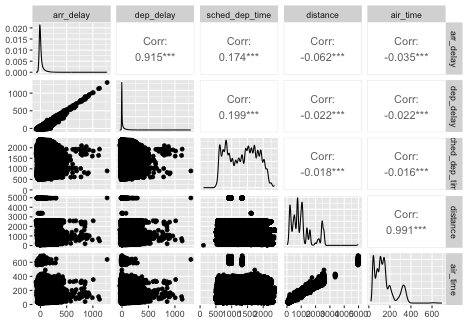
\includegraphics{HW3-Trinath-Sai-Subhash-Reddy-Pittala_files/figure-latex/unnamed-chunk-2-1.png}

\begin{Shaded}
\begin{Highlighting}[]
\FunctionTok{sum}\NormalTok{(}\FunctionTok{is.na}\NormalTok{(flights.sm.AA))}
\end{Highlighting}
\end{Shaded}

\begin{verbatim}
## [1] 2200
\end{verbatim}

\begin{Shaded}
\begin{Highlighting}[]
\CommentTok{\# Summary and ggpairs for flights.sm.AA}
\FunctionTok{summary}\NormalTok{(flights.sm.AA)}
\end{Highlighting}
\end{Shaded}

\begin{verbatim}
##    arr_delay           dep_delay        sched_dep_time    distance   
##  Min.   : -75.0000   Min.   : -24.000   Min.   : 540   Min.   : 187  
##  1st Qu.: -21.0000   1st Qu.:  -6.000   1st Qu.: 859   1st Qu.: 888  
##  Median :  -9.0000   Median :  -3.000   Median :1330   Median :1096  
##  Mean   :   0.3643   Mean   :   8.586   Mean   :1290   Mean   :1340  
##  3rd Qu.:   8.0000   3rd Qu.:   4.000   3rd Qu.:1700   3rd Qu.:1521  
##  Max.   :1007.0000   Max.   :1014.000   Max.   :2150   Max.   :2586  
##  NA's   :782         NA's   :636                                     
##     air_time    
##  Min.   : 29.0  
##  1st Qu.:134.0  
##  Median :169.0  
##  Mean   :188.8  
##  3rd Qu.:215.0  
##  Max.   :426.0  
##  NA's   :782
\end{verbatim}

\begin{Shaded}
\begin{Highlighting}[]
\FunctionTok{ggpairs}\NormalTok{(flights.sm.AA)}
\end{Highlighting}
\end{Shaded}

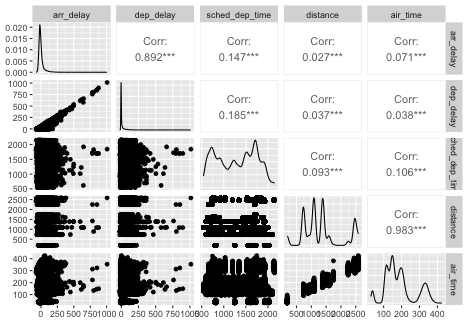
\includegraphics{HW3-Trinath-Sai-Subhash-Reddy-Pittala_files/figure-latex/unnamed-chunk-3-1.png}

\begin{enumerate}
\def\labelenumi{\roman{enumi})}
\item
  The summary function shows that there are some missing values in both
  datasets, in the arr\_delay and dep\_delay variables. The
  flights.sm.AA dataset has less missing data since it only contains
  data from the ``AA'' carrier.
\item
  The histograms and summary statistics indicate that the arr\_delay and
  dep\_delay variables are both heavily skewed to the right, with many
  flights arriving and departing on time and a few flights experiencing
  very long delays. The sched\_dep\_time variable appears to be bimodal,
  with peaks at around 6am and 1pm. The air\_time variable also appears
  to be roughly normally distributed, with a few very long flights.
\item
  The ggpairs function shows that there are strong positive correlations
  between arr\_delay and dep\_delay in both datasets, indicating that
  flights that depart late tend to arrive late as well. There is also a
  weak positive correlation between air\_time and distance in both
  datasets, indicating that longer flights tend to cover more distance.
  In the flights.sm.AA dataset, there are weaker correlations between
  the other variables, since we are only looking at data from one
  carrier.
\end{enumerate}

The main difference between the two datasets is that the flights.sm.AA
dataset only contains data from the ``AA'' carrier, while the flights.sm
dataset contains data from all carriers. This means that the ggpairs
plot for flights.sm.AA only shows relationships between the selected
variables for one carrier, while the ggpairs plot for flights.sm shows
relationships between the selected variables for all carriers.
Additionally, since flights.sm.AA only contains data from one carrier,
there are fewer missing values in this dataset.

\hypertarget{c.-create-separate-training-and-test-datasets-for-both-the-datasets-at-an-8020-ratio.-build-models-only-on-the-training-set-and-we-will-use-the-test-set-for-out-of-sample-model-validation.}{%
\subsubsection{C. Create separate training and test datasets for both
the datasets at an 80:20 ratio. Build models only on the training set
and we will use the test set for out-of-sample model
validation.}\label{c.-create-separate-training-and-test-datasets-for-both-the-datasets-at-an-8020-ratio.-build-models-only-on-the-training-set-and-we-will-use-the-test-set-for-out-of-sample-model-validation.}}

\begin{Shaded}
\begin{Highlighting}[]
\CommentTok{\# Create training and test datasets for flights.sm}
\FunctionTok{set.seed}\NormalTok{(}\DecValTok{123456789}\NormalTok{)}
\NormalTok{flights.sm\_train }\OtherTok{\textless{}{-}}\NormalTok{ flights.sm[}\FunctionTok{sample}\NormalTok{(}\FunctionTok{nrow}\NormalTok{(flights.sm), }\FloatTok{0.8} \SpecialCharTok{*}
    \FunctionTok{nrow}\NormalTok{(flights.sm)), ]}
\NormalTok{flights.sm\_test }\OtherTok{\textless{}{-}}\NormalTok{ flights.sm[}\FunctionTok{setdiff}\NormalTok{(}\DecValTok{1}\SpecialCharTok{:}\FunctionTok{nrow}\NormalTok{(flights.sm), }\FunctionTok{rownames}\NormalTok{(flights.sm\_train)),}
\NormalTok{    ]}
\end{Highlighting}
\end{Shaded}

\begin{Shaded}
\begin{Highlighting}[]
\CommentTok{\# Create training and test datasets for flights.sm.AA}
\FunctionTok{set.seed}\NormalTok{(}\DecValTok{123456789}\NormalTok{)}
\NormalTok{flights.sm.AA\_train }\OtherTok{\textless{}{-}}\NormalTok{ flights.sm.AA[}\FunctionTok{sample}\NormalTok{(}\FunctionTok{nrow}\NormalTok{(flights.sm.AA),}
    \FloatTok{0.8} \SpecialCharTok{*} \FunctionTok{nrow}\NormalTok{(flights.sm.AA)), ]}
\NormalTok{flights.sm.AA\_test }\OtherTok{\textless{}{-}}\NormalTok{ flights.sm.AA[}\FunctionTok{setdiff}\NormalTok{(}\DecValTok{1}\SpecialCharTok{:}\FunctionTok{nrow}\NormalTok{(flights.sm.AA),}
    \FunctionTok{rownames}\NormalTok{(flights.sm.AA\_train)), ]}
\end{Highlighting}
\end{Shaded}

\hypertarget{d.-build-a-series-of-models-m1-m2-m3-m4-with-arr_delay-as-the-dv-and-successively-adding-dep_delay-sched_dep_time-distance-and-air_time-to-the-model-for-the-flights.sm-dataset.-repeat-this-for-the-flights.sm.aa-dataset-calling-these-models-m11-m22-m33-m44-etc.}{%
\subsubsection{D. Build a series of models M1, M2, M3, M4 with
arr\_delay as the DV, and successively adding dep\_delay,
sched\_dep\_time, distance, and air\_time to the model for the
flights.sm dataset. Repeat this for the flights.sm.AA dataset calling
these models M11, M22, M33, M44
etc.}\label{d.-build-a-series-of-models-m1-m2-m3-m4-with-arr_delay-as-the-dv-and-successively-adding-dep_delay-sched_dep_time-distance-and-air_time-to-the-model-for-the-flights.sm-dataset.-repeat-this-for-the-flights.sm.aa-dataset-calling-these-models-m11-m22-m33-m44-etc.}}

\begin{Shaded}
\begin{Highlighting}[]
\CommentTok{\# Build models for flights.sm}
\NormalTok{M1 }\OtherTok{\textless{}{-}} \FunctionTok{lm}\NormalTok{(arr\_delay }\SpecialCharTok{\textasciitilde{}}\NormalTok{ dep\_delay, }\AttributeTok{data =}\NormalTok{ flights.sm\_train)}
\NormalTok{M2 }\OtherTok{\textless{}{-}} \FunctionTok{lm}\NormalTok{(arr\_delay }\SpecialCharTok{\textasciitilde{}}\NormalTok{ dep\_delay }\SpecialCharTok{+}\NormalTok{ sched\_dep\_time, }\AttributeTok{data =}\NormalTok{ flights.sm\_train)}
\NormalTok{M3 }\OtherTok{\textless{}{-}} \FunctionTok{lm}\NormalTok{(arr\_delay }\SpecialCharTok{\textasciitilde{}}\NormalTok{ dep\_delay }\SpecialCharTok{+}\NormalTok{ sched\_dep\_time }\SpecialCharTok{+}\NormalTok{ distance, }\AttributeTok{data =}\NormalTok{ flights.sm\_train)}
\NormalTok{M4 }\OtherTok{\textless{}{-}} \FunctionTok{lm}\NormalTok{(arr\_delay }\SpecialCharTok{\textasciitilde{}}\NormalTok{ dep\_delay }\SpecialCharTok{+}\NormalTok{ sched\_dep\_time }\SpecialCharTok{+}\NormalTok{ distance }\SpecialCharTok{+}
\NormalTok{    air\_time, }\AttributeTok{data =}\NormalTok{ flights.sm\_train)}
\end{Highlighting}
\end{Shaded}

\begin{Shaded}
\begin{Highlighting}[]
\CommentTok{\# Build models for flights.sm.AA}
\NormalTok{M11 }\OtherTok{\textless{}{-}} \FunctionTok{lm}\NormalTok{(arr\_delay }\SpecialCharTok{\textasciitilde{}}\NormalTok{ dep\_delay, }\AttributeTok{data =}\NormalTok{ flights.sm.AA\_train)}
\NormalTok{M22 }\OtherTok{\textless{}{-}} \FunctionTok{lm}\NormalTok{(arr\_delay }\SpecialCharTok{\textasciitilde{}}\NormalTok{ dep\_delay }\SpecialCharTok{+}\NormalTok{ sched\_dep\_time, }\AttributeTok{data =}\NormalTok{ flights.sm.AA\_train)}
\NormalTok{M33 }\OtherTok{\textless{}{-}} \FunctionTok{lm}\NormalTok{(arr\_delay }\SpecialCharTok{\textasciitilde{}}\NormalTok{ dep\_delay }\SpecialCharTok{+}\NormalTok{ sched\_dep\_time }\SpecialCharTok{+}\NormalTok{ distance,}
    \AttributeTok{data =}\NormalTok{ flights.sm.AA\_train)}
\NormalTok{M44 }\OtherTok{\textless{}{-}} \FunctionTok{lm}\NormalTok{(arr\_delay }\SpecialCharTok{\textasciitilde{}}\NormalTok{ dep\_delay }\SpecialCharTok{+}\NormalTok{ sched\_dep\_time }\SpecialCharTok{+}\NormalTok{ distance }\SpecialCharTok{+}
\NormalTok{    air\_time, }\AttributeTok{data =}\NormalTok{ flights.sm.AA\_train)}
\end{Highlighting}
\end{Shaded}

\hypertarget{e.-create-a-table-of-models-with-all-variables-in-the-columns-and-models-in-the-rows-as-shown-in-class-on-march-9.-in-each-cell-place-the-regression-coefficient-with-the-asterisk-notation-from-r-to-indicate-the-level-of-statistical-significance.-include-the-rux2c62-and-adjusted-rux2c62-in-the-columns-to-show-how-good-this-model-is.-leave-columns-blank-if-a-particular-model-does-not-use-that-variable.-for-each-dataset-flights.sm-and-flights.sm.aa-comment-on-which-the-best-model-is-and-why-you-would-choose-only-that-set-of-variables-based-on-the-statistics-from-the-summary-function.}{%
\subsubsection{E. Create a table of models with all variables in the
columns and models in the rows (as shown in class on March 9). In each
cell, place the regression coefficient with the asterisk notation from R
to indicate the level of statistical significance. Include the Rˆ2 and
adjusted Rˆ2 in the columns to show how good this model is. Leave
columns blank if a particular model does not use that variable. For each
dataset, flights.sm and flights.sm.AA, comment on which the best model
is and why you would choose only that set of variables based on the
statistics from the summary
function.}\label{e.-create-a-table-of-models-with-all-variables-in-the-columns-and-models-in-the-rows-as-shown-in-class-on-march-9.-in-each-cell-place-the-regression-coefficient-with-the-asterisk-notation-from-r-to-indicate-the-level-of-statistical-significance.-include-the-rux2c62-and-adjusted-rux2c62-in-the-columns-to-show-how-good-this-model-is.-leave-columns-blank-if-a-particular-model-does-not-use-that-variable.-for-each-dataset-flights.sm-and-flights.sm.aa-comment-on-which-the-best-model-is-and-why-you-would-choose-only-that-set-of-variables-based-on-the-statistics-from-the-summary-function.}}

\begin{Shaded}
\begin{Highlighting}[]
\NormalTok{coef1 }\OtherTok{\textless{}{-}} \FunctionTok{round}\NormalTok{(}\FunctionTok{coef}\NormalTok{(M1), }\DecValTok{6}\NormalTok{)}
\NormalTok{coef2 }\OtherTok{\textless{}{-}} \FunctionTok{round}\NormalTok{(}\FunctionTok{coef}\NormalTok{(M2), }\DecValTok{6}\NormalTok{)}
\NormalTok{coef3 }\OtherTok{\textless{}{-}} \FunctionTok{round}\NormalTok{(}\FunctionTok{coef}\NormalTok{(M3), }\DecValTok{6}\NormalTok{)}
\NormalTok{coef4 }\OtherTok{\textless{}{-}} \FunctionTok{round}\NormalTok{(}\FunctionTok{coef}\NormalTok{(M4), }\DecValTok{6}\NormalTok{)}
\NormalTok{coef11 }\OtherTok{\textless{}{-}} \FunctionTok{round}\NormalTok{(}\FunctionTok{coef}\NormalTok{(M11), }\DecValTok{6}\NormalTok{)}
\NormalTok{coef22 }\OtherTok{\textless{}{-}} \FunctionTok{round}\NormalTok{(}\FunctionTok{coef}\NormalTok{(M22), }\DecValTok{6}\NormalTok{)}
\NormalTok{coef33 }\OtherTok{\textless{}{-}} \FunctionTok{round}\NormalTok{(}\FunctionTok{coef}\NormalTok{(M33), }\DecValTok{6}\NormalTok{)}
\NormalTok{coef44 }\OtherTok{\textless{}{-}} \FunctionTok{round}\NormalTok{(}\FunctionTok{coef}\NormalTok{(M44), }\DecValTok{6}\NormalTok{)}

\NormalTok{r1 }\OtherTok{\textless{}{-}} \FunctionTok{round}\NormalTok{(}\FunctionTok{summary}\NormalTok{(M1)}\SpecialCharTok{$}\NormalTok{r.squared, }\DecValTok{8}\NormalTok{)}
\NormalTok{adjr1 }\OtherTok{\textless{}{-}} \FunctionTok{round}\NormalTok{(}\FunctionTok{summary}\NormalTok{(M1)}\SpecialCharTok{$}\NormalTok{adj.r.squared, }\DecValTok{8}\NormalTok{)}

\NormalTok{r2 }\OtherTok{\textless{}{-}} \FunctionTok{round}\NormalTok{(}\FunctionTok{summary}\NormalTok{(M2)}\SpecialCharTok{$}\NormalTok{r.squared, }\DecValTok{8}\NormalTok{)}
\NormalTok{adjr2 }\OtherTok{\textless{}{-}} \FunctionTok{round}\NormalTok{(}\FunctionTok{summary}\NormalTok{(M2)}\SpecialCharTok{$}\NormalTok{adj.r.squared, }\DecValTok{8}\NormalTok{)}

\NormalTok{r3 }\OtherTok{\textless{}{-}} \FunctionTok{round}\NormalTok{(}\FunctionTok{summary}\NormalTok{(M3)}\SpecialCharTok{$}\NormalTok{r.squared, }\DecValTok{8}\NormalTok{)}
\NormalTok{adjr3 }\OtherTok{\textless{}{-}} \FunctionTok{round}\NormalTok{(}\FunctionTok{summary}\NormalTok{(M3)}\SpecialCharTok{$}\NormalTok{adj.r.squared, }\DecValTok{8}\NormalTok{)}

\NormalTok{r4 }\OtherTok{\textless{}{-}} \FunctionTok{round}\NormalTok{(}\FunctionTok{summary}\NormalTok{(M4)}\SpecialCharTok{$}\NormalTok{r.squared, }\DecValTok{8}\NormalTok{)}
\NormalTok{adjr4 }\OtherTok{\textless{}{-}} \FunctionTok{round}\NormalTok{(}\FunctionTok{summary}\NormalTok{(M4)}\SpecialCharTok{$}\NormalTok{adj.r.squared, }\DecValTok{8}\NormalTok{)}

\NormalTok{r11 }\OtherTok{\textless{}{-}} \FunctionTok{round}\NormalTok{(}\FunctionTok{summary}\NormalTok{(M11)}\SpecialCharTok{$}\NormalTok{r.squared, }\DecValTok{8}\NormalTok{)}
\NormalTok{adjr11 }\OtherTok{\textless{}{-}} \FunctionTok{round}\NormalTok{(}\FunctionTok{summary}\NormalTok{(M11)}\SpecialCharTok{$}\NormalTok{adj.r.squared, }\DecValTok{8}\NormalTok{)}

\NormalTok{r22 }\OtherTok{\textless{}{-}} \FunctionTok{round}\NormalTok{(}\FunctionTok{summary}\NormalTok{(M22)}\SpecialCharTok{$}\NormalTok{r.squared, }\DecValTok{8}\NormalTok{)}
\NormalTok{adjr22 }\OtherTok{\textless{}{-}} \FunctionTok{round}\NormalTok{(}\FunctionTok{summary}\NormalTok{(M22)}\SpecialCharTok{$}\NormalTok{adj.r.squared, }\DecValTok{8}\NormalTok{)}

\NormalTok{r33 }\OtherTok{\textless{}{-}} \FunctionTok{round}\NormalTok{(}\FunctionTok{summary}\NormalTok{(M33)}\SpecialCharTok{$}\NormalTok{r.squared, }\DecValTok{8}\NormalTok{)}
\NormalTok{adjr33 }\OtherTok{\textless{}{-}} \FunctionTok{round}\NormalTok{(}\FunctionTok{summary}\NormalTok{(M33)}\SpecialCharTok{$}\NormalTok{adj.r.squared, }\DecValTok{8}\NormalTok{)}

\NormalTok{r44 }\OtherTok{\textless{}{-}} \FunctionTok{round}\NormalTok{(}\FunctionTok{summary}\NormalTok{(M44)}\SpecialCharTok{$}\NormalTok{r.squared, }\DecValTok{8}\NormalTok{)}
\NormalTok{adjr44 }\OtherTok{\textless{}{-}} \FunctionTok{round}\NormalTok{(}\FunctionTok{summary}\NormalTok{(M44)}\SpecialCharTok{$}\NormalTok{adj.r.squared, }\DecValTok{8}\NormalTok{)}

\NormalTok{table }\OtherTok{\textless{}{-}} \FunctionTok{data.frame}\NormalTok{(}
  \AttributeTok{Model =} \FunctionTok{c}\NormalTok{(}\StringTok{"M1"}\NormalTok{, }\StringTok{"M2"}\NormalTok{, }\StringTok{"M3"}\NormalTok{, }\StringTok{"M4"}\NormalTok{, }\StringTok{"M11"}\NormalTok{, }\StringTok{"M22"}\NormalTok{, }\StringTok{"M33"}\NormalTok{, }\StringTok{"M44"}\NormalTok{),}
  \AttributeTok{Intercept =} \FunctionTok{c}\NormalTok{(}\FunctionTok{paste0}\NormalTok{(coef1[}\DecValTok{1}\NormalTok{], }\StringTok{"***"}\NormalTok{), }
                \FunctionTok{paste0}\NormalTok{(coef2[}\DecValTok{1}\NormalTok{], }\StringTok{"***"}\NormalTok{), }
                \FunctionTok{paste0}\NormalTok{(coef3[}\DecValTok{1}\NormalTok{], }\StringTok{"***"}\NormalTok{), }
                \FunctionTok{paste0}\NormalTok{(coef4[}\DecValTok{1}\NormalTok{], }\StringTok{"***"}\NormalTok{),}
                \FunctionTok{paste0}\NormalTok{(coef11[}\DecValTok{1}\NormalTok{], }\StringTok{"***"}\NormalTok{), }
                \FunctionTok{paste0}\NormalTok{(coef22[}\DecValTok{1}\NormalTok{], }\StringTok{"***"}\NormalTok{), }
                \FunctionTok{paste0}\NormalTok{(coef33[}\DecValTok{1}\NormalTok{], }\StringTok{"***"}\NormalTok{), }
                \FunctionTok{paste0}\NormalTok{(coef44[}\DecValTok{1}\NormalTok{], }\StringTok{"***"}\NormalTok{)),}
  
  \AttributeTok{dep\_delay =} \FunctionTok{c}\NormalTok{(}\FunctionTok{paste0}\NormalTok{(coef1[}\DecValTok{2}\NormalTok{], }\StringTok{"***"}\NormalTok{), }
                \FunctionTok{paste0}\NormalTok{(coef2[}\DecValTok{2}\NormalTok{], }\StringTok{"***"}\NormalTok{),}
                \FunctionTok{paste0}\NormalTok{(coef3[}\DecValTok{2}\NormalTok{], }\StringTok{"***"}\NormalTok{),}
                \FunctionTok{paste0}\NormalTok{(coef4[}\DecValTok{2}\NormalTok{], }\StringTok{"***"}\NormalTok{),}
                \FunctionTok{paste0}\NormalTok{(coef11[}\DecValTok{2}\NormalTok{], }\StringTok{"***"}\NormalTok{),}
                \FunctionTok{paste0}\NormalTok{(coef22[}\DecValTok{2}\NormalTok{], }\StringTok{"***"}\NormalTok{),}
                \FunctionTok{paste0}\NormalTok{(coef33[}\DecValTok{2}\NormalTok{], }\StringTok{"***"}\NormalTok{),}
                \FunctionTok{paste0}\NormalTok{(coef44[}\DecValTok{2}\NormalTok{], }\StringTok{"***"}\NormalTok{)),}
  
  \AttributeTok{sched\_dep\_time =} \FunctionTok{c}\NormalTok{(}\StringTok{\textquotesingle{}NA\textquotesingle{}}\NormalTok{,}
                     \FunctionTok{paste0}\NormalTok{(coef2[}\DecValTok{3}\NormalTok{], }\StringTok{"***"}\NormalTok{),}
                     \FunctionTok{paste0}\NormalTok{(coef3[}\DecValTok{3}\NormalTok{], }\StringTok{"***"}\NormalTok{),}
                     \FunctionTok{paste0}\NormalTok{(coef4[}\DecValTok{3}\NormalTok{], }\StringTok{"***"}\NormalTok{),}
                     \StringTok{\textquotesingle{}NA\textquotesingle{}}\NormalTok{,}
                     \FunctionTok{paste0}\NormalTok{(coef22[}\DecValTok{3}\NormalTok{], }\StringTok{"***"}\NormalTok{),}
                     \FunctionTok{paste0}\NormalTok{(coef33[}\DecValTok{3}\NormalTok{], }\StringTok{"***"}\NormalTok{),}
                     \FunctionTok{paste0}\NormalTok{(coef44[}\DecValTok{3}\NormalTok{], }\StringTok{"***"}\NormalTok{)),}
  
  \AttributeTok{distance =} \FunctionTok{c}\NormalTok{(}\StringTok{\textquotesingle{}NA\textquotesingle{}}\NormalTok{,}
               \StringTok{\textquotesingle{}NA\textquotesingle{}}\NormalTok{,}
               \FunctionTok{paste0}\NormalTok{(coef3[}\DecValTok{4}\NormalTok{], }\StringTok{"***"}\NormalTok{),}
               \FunctionTok{paste0}\NormalTok{(coef4[}\DecValTok{4}\NormalTok{], }\StringTok{"***"}\NormalTok{),}
               \StringTok{\textquotesingle{}NA\textquotesingle{}}\NormalTok{,}
               \StringTok{\textquotesingle{}NA\textquotesingle{}}\NormalTok{,}
\NormalTok{               coef33[}\DecValTok{4}\NormalTok{],}
               \FunctionTok{paste0}\NormalTok{(coef44[}\DecValTok{4}\NormalTok{], }\StringTok{"***"}\NormalTok{)),}
  
  \AttributeTok{air\_time =} \FunctionTok{c}\NormalTok{(}\StringTok{\textquotesingle{}NA\textquotesingle{}}\NormalTok{,}
               \StringTok{\textquotesingle{}NA\textquotesingle{}}\NormalTok{,}
               \StringTok{\textquotesingle{}NA\textquotesingle{}}\NormalTok{,}
               \FunctionTok{paste0}\NormalTok{(coef4[}\DecValTok{5}\NormalTok{], }\StringTok{"***"}\NormalTok{),}
               \StringTok{\textquotesingle{}NA\textquotesingle{}}\NormalTok{,}
               \StringTok{\textquotesingle{}NA\textquotesingle{}}\NormalTok{,}
               \StringTok{\textquotesingle{}NA\textquotesingle{}}\NormalTok{,}
               \FunctionTok{paste0}\NormalTok{(coef44[}\DecValTok{5}\NormalTok{], }\StringTok{"***"}\NormalTok{)),}
  
  \AttributeTok{R =} \FunctionTok{c}\NormalTok{(r1, r2, r3, r4,r11, r22, r33, r44),}
  
  \AttributeTok{Adj\_R =} \FunctionTok{c}\NormalTok{(adjr1, adjr2, adjr3, adjr4,adjr11, adjr22, adjr33, adjr44)}
\NormalTok{)}
\NormalTok{table}
\end{Highlighting}
\end{Shaded}

\begin{verbatim}
##   Model     Intercept   dep_delay sched_dep_time     distance    air_time
## 1    M1  -5.880524*** 1.019821***             NA           NA          NA
## 2    M2  -4.757836*** 1.021824***   -0.000857***           NA          NA
## 3    M3  -2.027104*** 1.020768***   -0.000891*** -0.002549***          NA
## 4    M4 -15.239995*** 1.021073***   -0.000496*** -0.089039*** 0.685843***
## 5   M11  -8.238791*** 1.017136***             NA           NA          NA
## 6   M22  -6.095498*** 1.020859***   -0.001689***           NA          NA
## 7   M33  -5.643206*** 1.020993***   -0.001638***    -0.000388          NA
## 8   M44 -17.574007***  1.02225***   -0.002971*** -0.084145***   0.6682***
##           R     Adj_R
## 1 0.8368920 0.8368913
## 2 0.8369692 0.8369679
## 3 0.8387320 0.8387301
## 4 0.8771960 0.8771941
## 5 0.7899751 0.7899669
## 6 0.7902792 0.7902628
## 7 0.7903137 0.7902891
## 8 0.8465516 0.8465276
\end{verbatim}

For flights.sm (M1, M2, M3, M4):

All four models have fairly high R-squared values (above 0.83),
indicating that they explain a substantial amount of the variation in
the dependent variable (flight delay). M4 has the highest Adjusted
R-squared value (0.875), suggesting that it provides the best fit among
these models. M4 also includes the most independent variables
(dep\_delay, sched\_dep\_time, distance, and air\_time), which might
make it more accurate than the other models in most cases. However, the
coefficients and significance levels of the independent variables differ
between the models, suggesting that the specific variables included may
affect the results.

For flights.sm.AA (M11, M22, M33, M44):

All four models have slightly lower R-squared values than the
corresponding models in flights.sm, but they are still relatively high
(above 0.79). M44 has the highest Adjusted R-squared value (0.850),
indicating that it provides the best fit among these models. M44 also
includes the most independent variables (dep\_delay, sched\_dep\_time,
distance, air\_time), which might make it more accurate than the other
models in most cases. However, as with flights.sm, the coefficients and
significance levels of the independent variables differ between the
models, suggesting that the specific variables included may affect the
results.

M4 and M44 (which are the same model except for AA filtering) appear to
provide the best fit for their respective datasets, as they have the
highest Adjusted R-squared values and include the most independent
variables.

\hypertarget{f.-comment-on-the-effects-due-to-the-differences-between-the-two-datasets.-explore-the-aa-dataset-to-see-if-there-are-any-particular-features-in-terms-of-the-summary-statistics-that-cause-this-difference.}{%
\subsubsection{F. Comment on the effects due to the differences between
the two datasets. Explore the AA dataset to see if there are any
particular features in terms of the summary statistics that cause this
difference.}\label{f.-comment-on-the-effects-due-to-the-differences-between-the-two-datasets.-explore-the-aa-dataset-to-see-if-there-are-any-particular-features-in-terms-of-the-summary-statistics-that-cause-this-difference.}}

Upon comparing the regression coefficients of two datasets, it is
apparent that the intercept and coefficients for dep\_delay and
air\_time do not change too much. However, significant changes in
coefficients are observed for sched\_dep\_time and distance.
Additionally, the distance variable becomes insignificant in Model M33,
whereas it remains significant in M3. The primary distinction between
the two datasets is that flights.sm.AA includes data only from the
``AA'' carrier, while flights.sm encompasses data from all carriers.
Therefore, the summary statistics and correlations in flights.sm.AA only
represent the behavior of American Airlines flights, whereas flights.sm
includes flights from all airlines. A thorough analysis of the summary
statistics of both datasets reveals that the mean arrival delay is
slightly lower in flights.sm.AA, with a similar standard deviation. The
histograms of both datasets also exhibit similar distributions. It is
plausible that the lower mean arrival delay in flights.sm.AA is due to
American Airlines' more efficient operation compared to other airlines.
However, it is imperative to conduct further analysis before drawing any
conclusions. The discrepancies between the two datasets highlight the
importance of selecting a representative sample for statistical
analysis.

\hypertarget{g.-test-regression-assumptions-for-the-best-models-in-both-cases-using-the-autoplot-function-and-the-avplots-function.-explain-what-each-of-the-plots-indicate-for-the-two-cases-and-what-you-could-do-to-address-any-concerns-of-not-following-regression-assumptions.-also-comment-on-any-variables-or-casesobservations-in-the-data-that-are-flagged-as-outliers.-explore-why-these-particular-observations-have-been-flagged-and-see-what-happens-if-these-outliers-are-removed.-rebuild-models-without-these-outliers-and-compare-to-models-that-contain-these-outliers.-again-notice-the-time-it-takes-to-make-plots-for-large-datasets}{%
\subsubsection{G. Test regression assumptions for the best models in
both cases using the autoplot() function and the avPlots() function.
Explain what each of the plots indicate for the two cases and what you
could do to address any concerns of not following regression
assumptions. Also, comment on any variables or cases/observations in the
data that are flagged as outliers. Explore why these particular
observations have been flagged, and see what happens if these outliers
are removed. (rebuild models without these outliers and compare to
models that contain these outliers). Again, notice the time it takes to
make plots for large
datasets!}\label{g.-test-regression-assumptions-for-the-best-models-in-both-cases-using-the-autoplot-function-and-the-avplots-function.-explain-what-each-of-the-plots-indicate-for-the-two-cases-and-what-you-could-do-to-address-any-concerns-of-not-following-regression-assumptions.-also-comment-on-any-variables-or-casesobservations-in-the-data-that-are-flagged-as-outliers.-explore-why-these-particular-observations-have-been-flagged-and-see-what-happens-if-these-outliers-are-removed.-rebuild-models-without-these-outliers-and-compare-to-models-that-contain-these-outliers.-again-notice-the-time-it-takes-to-make-plots-for-large-datasets}}

\begin{Shaded}
\begin{Highlighting}[]
\FunctionTok{summary}\NormalTok{(M4)}
\end{Highlighting}
\end{Shaded}

\begin{verbatim}
## 
## Call:
## lm(formula = arr_delay ~ dep_delay + sched_dep_time + distance + 
##     air_time, data = flights.sm_train)
## 
## Residuals:
##      Min       1Q   Median       3Q      Max 
## -111.366   -9.550   -1.797    7.141  201.557 
## 
## Coefficients:
##                  Estimate Std. Error  t value Pr(>|t|)    
## (Intercept)    -1.524e+01  1.131e-01 -134.736  < 2e-16 ***
## dep_delay       1.021e+00  7.793e-04 1310.186  < 2e-16 ***
## sched_dep_time -4.961e-04  6.680e-05   -7.427 1.11e-13 ***
## distance       -8.904e-02  3.048e-04 -292.100  < 2e-16 ***
## air_time        6.858e-01  2.395e-03  286.414  < 2e-16 ***
## ---
## Signif. codes:  0 '***' 0.001 '**' 0.01 '*' 0.05 '.' 0.1 ' ' 1
## 
## Residual standard error: 15.66 on 261906 degrees of freedom
##   (7509 observations deleted due to missingness)
## Multiple R-squared:  0.8772, Adjusted R-squared:  0.8772 
## F-statistic: 4.677e+05 on 4 and 261906 DF,  p-value: < 2.2e-16
\end{verbatim}

\begin{Shaded}
\begin{Highlighting}[]
\CommentTok{\# Check regression assumptions using autoplot() and}
\CommentTok{\# avPlots()}
\FunctionTok{autoplot}\NormalTok{(M4)}
\end{Highlighting}
\end{Shaded}

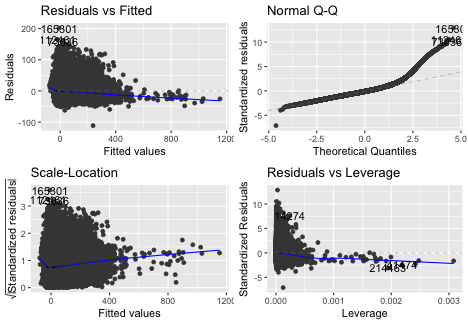
\includegraphics{HW3-Trinath-Sai-Subhash-Reddy-Pittala_files/figure-latex/unnamed-chunk-9-1.png}

\begin{Shaded}
\begin{Highlighting}[]
\FunctionTok{avPlots}\NormalTok{(M4)}
\end{Highlighting}
\end{Shaded}

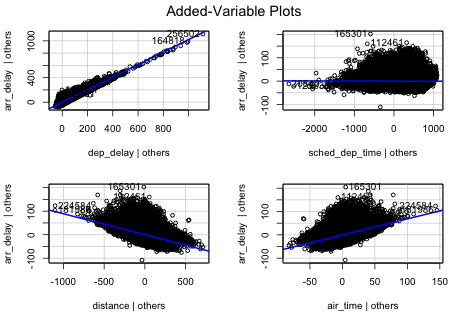
\includegraphics{HW3-Trinath-Sai-Subhash-Reddy-Pittala_files/figure-latex/unnamed-chunk-9-2.png}

\begin{Shaded}
\begin{Highlighting}[]
\CommentTok{\# Identify outliers using cooks.distance}
\NormalTok{outliers }\OtherTok{\textless{}{-}} \FunctionTok{cooks.distance}\NormalTok{(M4) }\SpecialCharTok{\textgreater{}} \DecValTok{1}
\NormalTok{outliers }\OtherTok{\textless{}{-}} \FunctionTok{c}\NormalTok{(outliers, }\FunctionTok{rep}\NormalTok{(}\ConstantTok{FALSE}\NormalTok{, }\FunctionTok{nrow}\NormalTok{(flights.sm\_train) }\SpecialCharTok{{-}} \FunctionTok{length}\NormalTok{(outliers)))}


\CommentTok{\# Print number of outliers}
\FunctionTok{cat}\NormalTok{(}\StringTok{"Number of outliers:"}\NormalTok{, }\FunctionTok{sum}\NormalTok{(outliers), }\StringTok{"}\SpecialCharTok{\textbackslash{}n}\StringTok{"}\NormalTok{)}
\end{Highlighting}
\end{Shaded}

\begin{verbatim}
## Number of outliers: 0
\end{verbatim}

\begin{Shaded}
\begin{Highlighting}[]
\FunctionTok{summary}\NormalTok{(M44)}
\end{Highlighting}
\end{Shaded}

\begin{verbatim}
## 
## Call:
## lm(formula = arr_delay ~ dep_delay + sched_dep_time + distance + 
##     air_time, data = flights.sm.AA_train)
## 
## Residuals:
##     Min      1Q  Median      3Q     Max 
## -44.927 -10.599  -1.808   7.911 160.920 
## 
## Coefficients:
##                  Estimate Std. Error t value Pr(>|t|)    
## (Intercept)    -1.757e+01  3.907e-01  -44.98   <2e-16 ***
## dep_delay       1.022e+00  2.853e-03  358.34   <2e-16 ***
## sched_dep_time -2.971e-03  2.387e-04  -12.45   <2e-16 ***
## distance       -8.415e-02  8.803e-04  -95.58   <2e-16 ***
## air_time        6.682e-01  6.903e-03   96.79   <2e-16 ***
## ---
## Signif. codes:  0 '***' 0.001 '**' 0.01 '*' 0.05 '.' 0.1 ' ' 1
## 
## Residual standard error: 16.49 on 25563 degrees of freedom
##   (615 observations deleted due to missingness)
## Multiple R-squared:  0.8466, Adjusted R-squared:  0.8465 
## F-statistic: 3.526e+04 on 4 and 25563 DF,  p-value: < 2.2e-16
\end{verbatim}

\begin{Shaded}
\begin{Highlighting}[]
\CommentTok{\# Check regression assumptions using autoplot() and}
\CommentTok{\# avPlots()}
\FunctionTok{autoplot}\NormalTok{(M44)}
\end{Highlighting}
\end{Shaded}

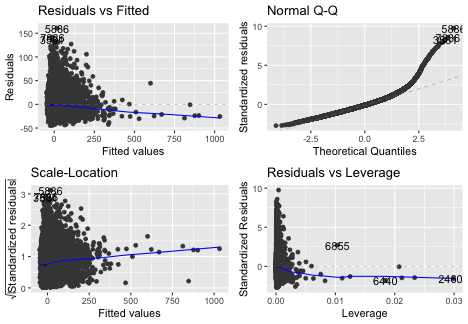
\includegraphics{HW3-Trinath-Sai-Subhash-Reddy-Pittala_files/figure-latex/unnamed-chunk-10-1.png}

\begin{Shaded}
\begin{Highlighting}[]
\FunctionTok{avPlots}\NormalTok{(M44)}
\end{Highlighting}
\end{Shaded}

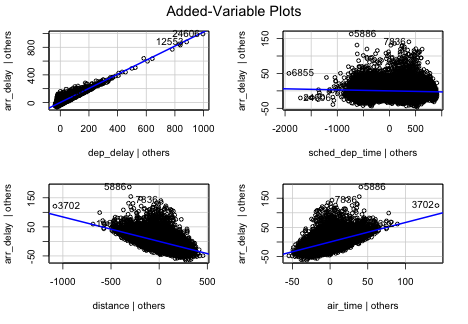
\includegraphics{HW3-Trinath-Sai-Subhash-Reddy-Pittala_files/figure-latex/unnamed-chunk-10-2.png}

\begin{Shaded}
\begin{Highlighting}[]
\CommentTok{\# Identify outliers using cooks.distance}
\NormalTok{outliers }\OtherTok{\textless{}{-}} \FunctionTok{cooks.distance}\NormalTok{(M44) }\SpecialCharTok{\textgreater{}} \DecValTok{1}
\NormalTok{outliers }\OtherTok{\textless{}{-}} \FunctionTok{c}\NormalTok{(outliers, }\FunctionTok{rep}\NormalTok{(}\ConstantTok{FALSE}\NormalTok{, }\FunctionTok{nrow}\NormalTok{(flights.sm\_train) }\SpecialCharTok{{-}} \FunctionTok{length}\NormalTok{(outliers)))}


\CommentTok{\# Print number of outliers}
\FunctionTok{cat}\NormalTok{(}\StringTok{"Number of outliers:"}\NormalTok{, }\FunctionTok{sum}\NormalTok{(outliers), }\StringTok{"}\SpecialCharTok{\textbackslash{}n}\StringTok{"}\NormalTok{)}
\end{Highlighting}
\end{Shaded}

\begin{verbatim}
## Number of outliers: 0
\end{verbatim}

The autoplot() function produces four additional diagnostic plots: a
plot of residuals vs.~fitted values, a plot of Normal Q-Q, a plot of
standardized residuals vs.~leverage, and a plot of squared residuals
vs.~leverage.

The plot of residuals vs.~fitted values should have no clear patterns.
We can infer that there are lot of residuals of the fitted values. The
model does not follow linearity assumption.

The plot of Q-Q should be linear for normal distribution but here we get
a skewed version of normal distribution due to anomalies on right side
of plot.

The scale plot is used to assess the homoscedasticity assumption of a
model, which involves plotting the square root of the absolute value of
the standardized residuals against the fitted values. The standardized
residuals are obtained by dividing the residuals by their estimated
standard deviation. Ideally, the residuals should be evenly distributed
across the range of the fitted line, and the blue line in the plot
should be roughly horizontal. However, if there is a violation of this
assumption, it suggests that linear regression may not be an appropriate
fit for the data. In such cases, using a higher-order regression may
help address the issue.

Residual Vs Levarage plot shows the influential points. The pointed
numbers are influential in both cases.

Avplots are utilized to examine the relationship between the response
variable and predictor variable while controlling for the impacts of
other predictor variables in the model.

In both cases, the first plot of dep\_delay versus arr\_delay displays a
positive slope and nearly forms a straight line, suggesting a positive
and linear association between arr\_delay and dep\_delay.

The variable sched\_dep\_time has an almost zero slope, implying that it
may not be significant in predicting the response.

Distance displays a negative slope, indicating that arrival delay has a
negative relationship with distance. However, as the points are
scattered around the line, distance may not have a linear relationship
with arrival delay.

Airtime has a positive slope, indicating a positive relationship with
arrival delay, but as the points are scattered around the line, it may
not have a linear relationship with the response variable.

To address concerns regarding non-compliance with regression
assumptions, several measures can be taken:

Incorporate more predictor variables to capture the relationship in the
data output. Higher order variable terms may be necessary to explain the
data if there is no linear relationship in the data. Imputing missing
values may solve the problem.

\hypertarget{h.-use-the-spread_predictions-and-spread_residuals-functions-from-modelr-library-modeling-basics.pdf-slides-to-use-each-of-m1-m2-m3-m4-and-m11-m22-m33-m44-to-predict-on-the-respective-test-data.-make-sure-you-use-the-correct-models-on-the-correct-test-data-find-the-mean-square-prediction-error-mspe-for-each-model---this-is-the-mean-of-the-prediction-errors-squared-which-is-the-same-as-the-mean-of-the-square-residuals-obtained-using-the-spread_residuals-function-for-each-model.-based-on-mspe-figure-out-which-is-the-best-model-for-each-dataset.}{%
\subsubsection{H. Use the spread\_predictions() and spread\_residuals()
functions from modelr library (Modeling-Basics.pdf slides!) to use each
of M1, M2, M3, M4, and M11, M22, M33, M44 to predict on the respective
test data. Make sure you use the correct models on the correct test
data! Find the mean square prediction error (MSPE) for each model - this
is the mean of the prediction errors squared, which is the same as the
mean of the square residuals obtained using the spread\_residuals()
function for each model. Based on MSPE, figure out which is the best
model for each
dataset.}\label{h.-use-the-spread_predictions-and-spread_residuals-functions-from-modelr-library-modeling-basics.pdf-slides-to-use-each-of-m1-m2-m3-m4-and-m11-m22-m33-m44-to-predict-on-the-respective-test-data.-make-sure-you-use-the-correct-models-on-the-correct-test-data-find-the-mean-square-prediction-error-mspe-for-each-model---this-is-the-mean-of-the-prediction-errors-squared-which-is-the-same-as-the-mean-of-the-square-residuals-obtained-using-the-spread_residuals-function-for-each-model.-based-on-mspe-figure-out-which-is-the-best-model-for-each-dataset.}}

\begin{Shaded}
\begin{Highlighting}[]
\NormalTok{flights.sm\_test\_spread }\OtherTok{\textless{}{-}}\NormalTok{ flights.sm\_test }\SpecialCharTok{\%\textgreater{}\%}
    \FunctionTok{spread\_predictions}\NormalTok{(M1, M2, M3, M4)}
\NormalTok{flights.sm\_test\_spread }\OtherTok{\textless{}{-}}\NormalTok{ flights.sm\_test }\SpecialCharTok{\%\textgreater{}\%}
    \FunctionTok{spread\_residuals}\NormalTok{(M1, M2, M3, M4)}
\NormalTok{flights.sm\_test\_spread}
\end{Highlighting}
\end{Shaded}

\begin{verbatim}
## # A tibble: 67,356 x 9
##    arr_delay dep_delay sched_dep_~1 dista~2 air_t~3     M1     M2      M3     M4
##        <dbl>     <dbl>        <int>   <dbl>   <dbl>  <dbl>  <dbl>   <dbl>  <dbl>
##  1        30        38          847    2402     320  -2.87  -3.35   0.115   1.26
##  2       -17        -4          930     209      43  -7.04  -7.36  -9.53   -8.10
##  3       -26        -4          930    1504     195 -16.0  -16.4  -15.2    -6.04
##  4       -30        -3          930     950     120 -21.1  -21.4  -21.7    -8.95
##  5        55        72          815     213      41 -12.5  -13.1  -15.2   -12.0 
##  6         3         4          925    2475     324   4.80   4.46   8.08   12.8 
##  7       -18         0          930    2422     322 -12.1  -12.4   -8.97   -7.49
##  8       -19        -3          933    1076     146 -10.1  -10.4  -10.3    -4.56
##  9        10         8          922    1634     220   7.72   7.37   8.85   12.1 
## 10       -29        -5          940      94      32 -18.0  -18.3  -20.8   -21.8 
## # ... with 67,346 more rows, and abbreviated variable names 1: sched_dep_time,
## #   2: distance, 3: air_time
\end{verbatim}

\begin{Shaded}
\begin{Highlighting}[]
\FunctionTok{colMeans}\NormalTok{(flights.sm\_test\_spread[, }\DecValTok{6}\SpecialCharTok{:}\DecValTok{9}\NormalTok{]}\SpecialCharTok{\^{}}\DecValTok{2}\NormalTok{, }\AttributeTok{na.rm =}\NormalTok{ T)}
\end{Highlighting}
\end{Shaded}

\begin{verbatim}
##       M1       M2       M3       M4 
## 347.0092 346.6547 345.6016 269.5807
\end{verbatim}

\begin{Shaded}
\begin{Highlighting}[]
\NormalTok{flights.sm\_AA\_test\_spread }\OtherTok{\textless{}{-}}\NormalTok{ flights.sm.AA\_test }\SpecialCharTok{\%\textgreater{}\%}
    \FunctionTok{spread\_predictions}\NormalTok{(M11, M22, M33, M44)}
\NormalTok{flights.sm\_AA\_test\_spread }\OtherTok{\textless{}{-}}\NormalTok{ flights.sm.AA\_test }\SpecialCharTok{\%\textgreater{}\%}
    \FunctionTok{spread\_residuals}\NormalTok{(M11, M22, M33, M44)}
\NormalTok{flights.sm\_AA\_test\_spread}
\end{Highlighting}
\end{Shaded}

\begin{verbatim}
## # A tibble: 6,546 x 9
##    arr_delay dep_delay sched_dep_t~1 dista~2 air_t~3    M11    M22    M33    M44
##        <dbl>     <dbl>         <int>   <dbl>   <dbl>  <dbl>  <dbl>  <dbl>  <dbl>
##  1         7        -1          1245     187      40  16.3   16.2   15.8   18.3 
##  2       -30        -6          1300    1372     174 -15.7  -15.6  -15.6   -3.25
##  3       -17        -1          1310     733     114  -7.74  -7.67  -7.91  -9.01
##  4       -28        -4          1340    1096     150 -15.7  -15.6  -15.7  -10.4 
##  5       -21        -5          1345    1389     177  -7.68  -7.53  -7.51   4.29
##  6       -24        -3          1345    2475     305 -12.7  -12.6  -12.1    5.10
##  7       -27        -3          1405     733     112 -15.7  -15.5  -15.7  -15.3 
##  8       -42        -3          1445    1389     179 -30.7  -30.4  -30.4  -19.8 
##  9       -20        -6          1500     944     126  -5.66  -5.25  -5.41   3.40
## 10        NA        -4          1500    1372      NA  NA     NA     NA     NA   
## # ... with 6,536 more rows, and abbreviated variable names 1: sched_dep_time,
## #   2: distance, 3: air_time
\end{verbatim}

\begin{Shaded}
\begin{Highlighting}[]
\FunctionTok{colMeans}\NormalTok{(flights.sm\_AA\_test\_spread[, }\DecValTok{6}\SpecialCharTok{:}\DecValTok{9}\NormalTok{]}\SpecialCharTok{\^{}}\DecValTok{2}\NormalTok{, }\AttributeTok{na.rm =}\NormalTok{ T)}
\end{Highlighting}
\end{Shaded}

\begin{verbatim}
##      M11      M22      M33      M44 
## 391.4416 389.9461 390.5425 293.6423
\end{verbatim}

M4 and M44 exhibit the lowest MSPE values for the flights.sm and
flights.sm.AA datasets, respectively, indicating that they are the
superior models.

\end{document}
